\clearpage{\pagestyle{empty}\cleardoublepage}
%%%%%%%%%%%%%%%%%%%%%%%%%%%%%%%%%%%%%%%%%imposta l'intestazione di pagina
\lhead[\fancyplain{}{\bfseries\thepage}]{\fancyplain{}{\bfseries\rightmark}}
\pagenumbering{arabic}                  %mette i numeri arabi
\chapter{Stato dell'arte}

I \textit{metadati} sono informazioni associate ad una pagina web o ad una porzione di essa che ne descrivono il contenuto, permettendo che i risultati delle ricerche degli utenti abbiano una maggiore efficacia.

Generare metadati di buona qualità in modo efficiente è essenziale per organizzare e rendere accessibile la grande quantità di risorse presente sul web. Il successo di biblioteche digitali, il sostenimento dell'interoperabilità e l'evoluzione del web semantico dipendono da una generazione di metadati efficiente\cite{metadata}.

\vspace{5mm}

L'utilizzo di strumenti automatici di generazione di metadati può facilitare la gestione di una quantità sempre crescente di informazioni.
Idealmente, questi strumenti sono capaci di estrarre informazioni da risorse strutturate e non strutturate, creando metadati di qualità che possano permettere interoperabilità semantica.

\vspace{5mm}

Tra i benifici delle generazione automatica di metadati vi è la scalabilità, per coprire la metadatazione di grandi quantità di informazioni che richiederebbe molto tempo se venisse gestita tutta manualmente, e la consistenza nella generazione dei dati.

\subsection{Metodi di generazione automatica}

A differenza della generazione manuale dei metadati, la generazione automatica dei metadati si basa su metodi automatici per assistere o completare il processo di creazione dei metadati. Greenberg ha distinto due metodi di generazione automatica dei metadati: l'estrazione dei metadati (\textit{metadata extraction}) e la raccolta dei metadati (\textit{metadata harvesting}).
L'estrazione dei metadati utilizza l'indicizzazione automatica e le tecniche di recupero delle informazioni per generare metadati strutturati utilizzando il contenuto originale delle risorse. La raccolta di metadati consiste invece nel raccogliere in modo automatico metadati già prodotti e archiviati da diversi repository.

\vspace{5mm}

All'interno di questa dicotomia di metodi di estrazione, vi sono molte tecniche più specifiche che i ricercatori hanno sviluppato per la generazione automatica di metadati. Polfreman et al. ha identificato sei tecniche che sono state sviluppate nel corso degli anni: raccolta di meta-tag, estrazione di contenuti, indicizzazione automatica, text e data mining, autogenerazione di dati estrinseci e social tagging. Sebbene l'ultima tecnica non sia propriamente una tecnica di generazione automatica di metadati, poiché viene utilizzata per generare metadati con un intervento minimo richiesto dai professionisti dei metadati, può essere vista come una possibile modalità per semplificare il processo di creazione dei metadati\cite{semi}.

\subsubsection{Estrazione di meta-tag}
L'\textbf{estrazione di meta-tag} è un processo dove vengono identificati valori per campi di metadati e popolati attraverso l'osservazione dei tag associati ai documenti, di fatto convertendo i metadati raccolti da più repository in formati diversi.

La più grande debolezza di questo tipo di tool è il fatto che la sua efficacia dipenda dalla qualità dei metadati raccolti.
Tra i tool che sfruttano questa tecnica vi sono MarcEdit, che mediante appositi harvester raccoglie metadati da record conformi al protocollo \textbf{Open Archives Initiative Protocol for Metadata Harvesting} (\textbf{OAI-PMH}) e che può convertire in diversi formati (MARC, MARC XML, MODS, EAD), e tool come Editor-Converter Dublin Core Metadata e Firefox Dublin Core Viewer Extension che convertono informazioni trovate nei meta-tags dei file HTML trovati sul web in elementi Dublin Core.

L'OAI-PMH fornisce un framework di interoperabilità, indipendente dall'applicazione, basata sul raccoglimento dei metadati. Il framework di OAI-PMH comprende i service provider, che eseguono richieste per effettuare la raccolta dei metadati, e i data provider, che espongono i metadati. OAI-PMH è largamente utilizzato da biblioteche digitale, repository istituzionali e archivi digitali\cite{harvesting}. Alcuni esempi di archivi che implementano OAI-PMH sono:

\begin{itemize}
\item Digital Public Library of America (DPLA), aggrega metadati relativi a enti istituzionali americani
\item National Science Digital Library (NSDL), è un libreria digitale ad accesso libero contenente collezioni di metadati inerenti a scienze, tecnologia, ingegneria e matematica
\item OAIster, un catalogo di milioni di record relativi a risorse di fonti eterogenee
\item Open Language Archives Community (OLAC), una libreria virtuale di risorse linguistiche
\end{itemize}

\subsubsection{Estrazione di contenuti}
L'\textbf{estrazione di contenuti} è una forma di estrazione di metadati che sfrutta algoritmi di machine learning per associare parole chiave al documento sulla base del suo contenuto. Il vantaggio di questo approccio è che il risultato è indipendente dalla qualità dei metadati associati alla risorsa. Esempi di applicazioni che impiegano questa tecnica sono Kea, che utilizza le tecniche TF-IDF e first-occurence per identificare e assegnare frasi chiave da risorse testuali, e Open Text Summarizer che esegue l'estrazione automatica di un riassunto del testo passato in input e delle relative parole chiave. 

I metodi di estrazione di parole chiave possono essere suddivisi in tre categorie: metodi statistici, metodi basati sui grafi e metodi basati sul deep learning\cite{extraction}.

\paragraph{Metodi statistici}
I \textbf{metodi statistici} sono i più semplici. Calcolano le statistiche per le parole chiave e utilizzano tali statistiche per valutarle. Tra questi metodi rientrano il calcolo la frequenza delle parole, la collocazione linguistica, la co-occorrenza e tecniche più sofisticate come TF-IDF e YAKE!.

\textbf{TF-IDF} (Term Frequency–Inverse Document Frequency) stima l'importanza della parola nel documento rispetto all'intero corpus (insieme di più documenti). Calcola la frequenza di ogni termine nel documento e la pondera con l'inverso della frequenza del termine nell'intero corpus. Le parole chiave verranno selezionate tra i termini con i punteggi più alti. Questo algoritmo favorisce i termini frequenti nel documento di testo e non frequenti negli altri documenti. Il vantaggio di TF-IDF è che è veloce e lo svantaggio è che necessita di un corpus di almeno qualche dozzina di documenti. TF-IDF è indipendente dalla lingua.

\textbf{YAKE!} (Yet Another Keyword Extractor) è un metodo di estrazione di parole chiave che utilizza funzionalità statistiche ricavate da un singolo documento per estrarre le parole chiave. Estrae le parole chiave in cinque passaggi:
\begin{enumerate}
\item \textbf{Pre-elaborazione e identificazione del termine candidato}: il testo è suddiviso in frasi, blocchi (parte della frase separata da punteggiatura) e token. Il testo viene pulito, etichettato e vengono identificate le stop words.
\item \textbf{Estrazione delle caratteristiche}: calcola le seguenti cinque caratteristiche statistiche per i termini (parole) nel documento:
\begin{itemize}
\item Casing: conta il numero di volte (in proporzionale al numero complessivo di volte in cui compare) in cui il termine appare in maiuscolo o come acronimo nel testo. Un termine significativo di solito appare più spesso in maiuscolo.
\item Posizione del termine: posizione mediana della frase del termine nel testo. I termini più vicini all'inizio tendono a essere i più significativi.
\item Normalizzazione della frequenza dei termini: misura la frequenza equilibrata dei termini nel documento.
\item Relazione del termine al contesto: misura con quanti termini diversi il termine candidato coesiste. Termini più significativi coesistono con termini meno diversi. 
\item Termine in frasi diverse: misura quante volte i termini compaiono in frasi diverse. Un punteggio più alto indica un termine più significativo.
\end{itemize}
\item \textbf{Calcolo del punteggio del termine}: le funzioni del passaggio precedente vengono combinate in un unico punteggio con l'equazione creata dall'uomo.
\item \textbf{Generazione di n-grammi e calcolo dei punteggi delle parole chiave}: l'algoritmo identifica tutti gli n-grammi validi. Le parole negli n-grammi devono appartenere allo stesso blocco e non devono iniziare o terminare con una stopword. Successivamente, ogni n-grammo viene valutato moltiplicando i punteggi dei suoi membri e normalizzato per ridurre l'impatto della lunghezza di n-gram. Le stopword vengono trattate in modo diverso per ridurre al minimo il loro impatto.
\item \textbf{Deduplicazione e ranking dei dati}: vengono rimosse le parole chiavi simili tra loro.
\end{enumerate}

\paragraph{Metodi basati sui grafi}
I metodi basati su grafi generano un grafo dei termini correlati presenti nei documenti. Un grafo, ad esempio, può collegare i termini che si verificano contemporaneamente nel testo. I metodi basati su grafi utilizzano metodi di classificazione che considerano la struttura del grafo per valutare l'importanza del vertice. Uno dei metodi di questa categoria più conosciuti è TextRank.

\textbf{TextRank} è un metodo di classificazione basato su grafi utilizzato per estrarre frasi pertinenti o trovare parole chiave. L'estrazione delle parole chiave avviene in cinque passaggi:

\begin{itemize}
\item Tokenizzazione e annotazione del testo con tag di Part of Speech (PoS) (nomi, articoli, verbi...)
\item Costruzione del grafo di co-occorrenza di parole: i vertici nel grafo sono parole con tag PoS selezionati. Due vertici sono collegati con un bordo se compaiono all'interno della finestra di N parole nel testo. Il grafo è non orientato e non ponderato.
\item Graph ranking: il punteggio di ciascun vertice è impostato su 1 e l'algoritmo di ranking viene eseguito sul grafo. L'algoritmo utilizza la seguente equazione:
\begin{equation}
S(Vi)=(1 - d) + d\left (\sum_{j \in In(Vi)} \frac{S(Vk)}{|Out(Vk)|}\right )
\end{equation}
Il peso S(Vi) di un vertice Vi è calcolato considerando i pesi dei vertici connessi al nodo Vi. Nell'equazione, d è il fattore di smorzamento impostato su 0,85, come suggerito nell'articolo di PageRank. In(Vi) sono collegamenti in entrata al vertice Vi e Out(Vj) sono collegamenti in uscita dal vertice Vj. Poiché stiamo considerando grafi non orientati, i collegamenti in entrata del vertice e i collegamenti in uscita del vertice sono gli stessi. L'algoritmo viene eseguito su ciascun nodo in diverse iterazioni fino a quando i pesi sui nodi convergono: la variazione tra le iterazioni è inferiore a 0,0001.
\item Selezione delle parole con il punteggio più alto: le parole (quindi i vertici) sono ordinate dalle parole con il punteggio più alto a quelle con il punteggio più basso. Alla fine, l'algoritmo seleziona il primo terzo delle parole.
\item Estrazione delle parole chiave: in questo passaggio, le parole selezionate nella fase precedente vengono unite in parole chiave composte da più parole se compaiono insieme nel testo. Il punteggio delle parole composte corrisponde alla somma dei punteggi delle parole singole che le compongono.
\end{itemize}

L'algoritmo viene eseguito su ciascun documento separatamente e non necessita di un corpus di documenti per eseguire l'estrazione delle parole chiave. TextRank è indipendente dalla lingua.

\textbf{RAKE} (Rapid Automatic Keyword Extraction) è un altro algoritmo di estrazione delle parole chiave basato su grafi. L'algoritmo si basa sull'osservazione che le parole chiave sono spesso composte da più parole e di solito non includono stop-word o punteggiatura.

Include i seguenti passaggi:
\begin{itemize}
\item Estrazione delle parole chiave candidate: il testo viene suddiviso in base alle parole chiave candidate in base alle parole di arresto e al delimitatore di frase. Una parola chiave candidata è una frase che si trova tra due stop-word o delimitatori di frase. I delimitatori di frase sono, ad esempio, i caratteri di punteggiatura.
\item Parole chiave costruzione del grafo di co-occorrenza: i vertici nel grafo sono parole. Sono collegati se compaiono insieme nelle parole chiave candidate. Il grafo è ponderato: il peso corrisponde al numero di volte in cui le parole collegate appaiono insieme nelle parole chiave candidate. Il grafo include anche le connessioni al vertice stesso (ogni parola appare in una parola chiave candidata con se stessa).
\item Punteggio delle parole: ogni parola nel grafo è valutata con uno dei seguenti punteggi: 
\begin{itemize}
\item Grado della parola deg(w): numero di parole con cui la parola w co-occorre (somma dei pesi degli archi). Il grado favorisce le parole che compaiono più spesso e in parole chiave più lunghe.
\item Frequenza della parola freq(w): numero di volte che la parola appare in qualsiasi parola chiave candidata. Questo criterio favorisce le parole che appaiono più frequentemente.
\item Rapporto tra grado e frequenza deg(w)/freq(w): favorisce le parole che ricorrono principalmente nelle parole chiave candidate più lunghe. Il grado favorirà le parole chiave più brevi.
\end{itemize}
\item Punteggio delle parole chiave candidate: il punteggio di ciascuna parola chiave candidata è la somma dei punteggi delle parole dei membri.
\item Parole chiave adiacenti: le parole chiave candidate non includono parole non significative. Poiché a volte le parole non significative possono essere parte della parola chiave, vengono aggiunte in questo passaggio. L'algoritmo trova coppie di parole chiave unite con una parola non significativa in un testo e le aggiunge all'insieme di parole non significative esistenti. Devono apparire almeno due volte nel testo da aggiungere. Il punteggio della nuova parola chiave è la somma delle parole chiave dei suoi membri.
\item Estrazione delle parole chiave: di conseguenza, viene estratto un terzo delle parole chiave con il punteggio migliore.
\end{itemize}

La differenza principale tra RAKE e TextRank è che RAKE considera le ricorrenze all'interno delle parole chiave candidate invece di una finestra fissa. Utilizza una procedura di punteggio più semplice e statistica: non include l'ottimizzazione. L'algoritmo viene eseguito su ciascun documento separatamente, quindi non necessita di un corpus di documenti.

\paragraph{Metodi basati sul deep learning}
La comparsa del deep learning ha consentito metodi basati sull'embedding, un insieme di tecniche di modellazione in cui le parole vengono mappate in vettori di numeri reali. 

Questi metodi trovano principalmente un elenco di parole chiave candidate (ad esempio, Bennani et al. considerano solo parole chiave costituite da nomi e aggettivi). Incorporano il documento e le parole chiave candidate nello stesso spazio di inclusione e misurano la similarità (ad es. similarità del coseno) tra i valori del documento e delle parole chiave. Selezionano le parole chiave più simili al testo del documento in base alla misura di similarità.

\subsubsection{Indicizzazione automatica}
Così come la content extraction, l'\textbf{indicizzazione automatica} prevede l'utilizzo di machine learning e algoritmi rule-based per estrarre metadati dalle risorse. La differenza sta nel fatto che i termini estratti vengono successivamente mappati in vocabolari controllati come Library of Congress Subject Headings (LCSH), Getty Thesaurus of Geographic Names (TGN), Library of Congress Name Authority (LCNA) o ontologie relative a un dominio specifico.

\subsubsection{Text e data mining}
A causa della complessità delle tecniche utilizzate per l'estrazione di metadati, la maggior parte degli usi di queste tecniche sono stati sviluppati per risolvere i problemi della generazione automatica di metadati nel contesto di specifici progetti di ricerca.
I principali motivi sono il fatto che l'efficacia di queste tecniche dipende dalla qualità e dalla quantità dei dati di training, e che i vocabolari controllati come LCSH sono troppo complicati e diversificati per essere applicati con mezzi automatici.

\subsubsection{Autogenerazione di dati estrinseci}
La generazione automatica di dati estrinseci è il processo di estrazione dei metadati su una risorsa informativa che non è contenuta all'interno della risorsa stessa. La generazione automatica di dati estrinseci può includere l'estrazione di metadati tecnici come il formato e le dimensioni del file, ma può essere anche l'estrazione di funzionalità più complesse come il livello di classe scolastica a cui è destinata una risorsa educativa o il tipo di lettori per cui è destinato un documento.
Processi di questo tipo sono difficili da implementare a causa dell'assenza di informazioni sul contesto di una risorsa
contenute nella risorsa stessa.
Tra i tool che implementano questa tecnica di estrazione di metadati vi sono Dspace e JHove.

\subsubsection{Social Tagging}
Il social tagging è una forma di generazione di metadati, sebbene non propriamente automatica, che permette agli utenti di creare e assegnare tag alle risorse di un sito web. A causa del costo relativamente basso della generazione e del mantenimento dei metadati attraverso il social tagging e della sua attuale popolarità diffusa, alcuni progetti hanno tentato di utilizzare questi dati per migliorare i repository di archiviazione di metadati. Ad esempio, Linstaedt et al. usa sofisticati programmi per computer per analizzare le immagini statiche trovate all'interno di Flickr e utilizzare questi risultati d'analisi per propagare tag utente pertinenti a nuove immagini elaborate.

Un esempio di utilizzo del social tagging più complesso può consistere nell'utilizzare tecniche di apprendimento automatico, tenendo traccia dei cambiamenti applicati sui metadati associati a una risorsa da parte degli utenti e migliorare quindi i meccanismi di learning del database sulla base di queste modifiche.
Tra i tool che supportano il social tagging vi sono Dspace e Omeka.

Sebbene gli strumenti di generazione automatica di metadati offrano molti vantaggi, soprattutto per quanto riguarda la semplificazione del processo di creazione dei metadati, esistono barriere significative all'adozione e all'implementazione diffusa di questi strumenti. Un problema incontrato con gli strumenti di generazione automatica di metadati è che molti di essi sono sviluppati localmente per soddisfare le esigenze specifiche di un determinato progetto o come parte della ricerca accademica.

Diversi tool sono focalizzati alla risoluzione di pochi problemi specifici legati alla generazione di metadati, come possono essere l'estrazione di parole chiave di Kea piuttosto che l'estrazione di tag HTML e la successiva conversione in elementi Dublin Core di Editor Converter Dublin Core, portando quindi a sforzi significativi per coordinare le applicazioni selezionate e ottenere l'output desiderato.
È inoltre necessaria una buona conoscenza tecnica di linguaggi di programmazione per implementare questi sistemi propriamente.

Un altro problema è la discontinuità delle applicazioni, che possono presto risultare obsolete e perdere supporto tecnico.

\section{Ricerca sul tema}
Gli sforzi di ricerca per la generazione automatica di metadati possono essere classificati in due aree: \textbf{ricerca sperimentale}, focalizzata sulle tecniche di recupero delle informazioni e sui contenuti delle risorse digitali, e \textbf{ricerca applicativa}, riguardante lo sviluppo di software per la creazione di contenuti e strumenti di generazione di metadati utilizzati nel contesto operativo\cite{amega}.

\subsection{Ricerca sperimentale}
La crescita dei repository di risorse digitali fornisce una grande quantità di collezioni per lo studio della generazione automatica di metadati.

I ricercatori che gestiscono il contenuto delle risorse digitali per la generazione di metadati hanno sperimentato principalmente con la \textbf{struttura dei documenti} e i \textbf{sistemi di rappresentazione della conoscenza}.

\subsubsection{Struttura del documento}
I ricercatori hanno identificato relazioni tra genere, contenuto e struttura del documento. Ad esempio, il genere del documento può dare informazioni sulla densità testuale, che può essere utilizzata per prevedere le prestazioni dell'algoritmo di estrazione dei metadati per determinati tipi di documenti.

Il genere del documento inoltre determina una struttura prevedibile che facilita l'estrazione automatica di metadati. Ad esempio, i documenti di ricerca includono informazioni standard come "titolo", "autore" e "affiliazione dell'autore del documento. Gli esperimenti che sfruttano la struttura del documento in questa seconda sede utilizzando un algoritmo Support Vector Machine (SVM) (ad esempio, Han et al., 2003) e Variable Hidden Markov Model (DVHMM) (Takasu, 2003) hanno avuto un discreto successo per la generazione di metadati.

\subsubsection{Sistemi di rappresentazione della conoscenza}
La memorizzazione di metadati può essere eseguita attraverso l'utilizzo di ontologie, thesauri, sistemi classificatori, file di autorità e altri strumenti di rappresentazione della conoscenza.
Attraverso l'utilizzo di regole di inferenza, è possibile generare ulteriori informazioni relative a un oggetto sulla base dei valori delle sue proprietà.

\subsection{Ricerca applicativa}
Tra gli strumenti in grado di generare automaticamente metadati è possibile distinguere i software per la creazione di contenuti da tool più specializzati conosciuti come applicazioni per la generazione di metadati.

\subsubsection{Software per la creazione di contenuti}
Esempi di software per la creazione di contenuti sono Microsoft Word, Adobe Acrobat e Nullsoft Winamp, essenzialmente qualsiasi software che può essere utilizzato per creare contenuti digitali, testuali o multimediali. Nel contesto del web, il software per la creazione di contenuti viene utilizzato per creare una risorsa digitale a cui è possibile accedere tramite un browser e il software associato. Anche un surrogato bibliografico può essere considerato contenuto.

I software per la creazione di contenuti possono supportare la generazione di metadati tramite mezzi automatici, semiautomatici e umani. Le tecniche automatiche sono spesso impiegate per produrre metadati tecnici come la data di creazione, la data dell'ultima modifica, la dimensione in byte e il formato del file.

Alcuni software per la creazione di contenuti estraggono i metadati dal contenuto del documento nel tentativo di fornire rappresentazioni descrittive (ad esempio, Word assegna automaticamente un titolo in base alla prima riga di un documento). Alcuni software per la creazione di contenuti includono un modello per facilitare l'immissione di metadati umani. Le tecniche automatiche possono quindi essere impiegate dall'applicazione per convertire i metadati immessi in un linguaggio di codifica specificato, incorporarli in un'intestazione di risorsa o inserirli in un database di metadati.

\subsubsection{Applicazioni e generazione automatica di metadati}
Le applicazioni per la generazione di metadati differiscono dal software per la creazione di contenuti in quanto sono progettate specificamente e solo per produrre record di metadati. 
La quantità di elaborazione automatica e umana richiesta per produrre metadati distingue i generatori, applicazioni che si basano principalmente su tecniche automatiche, dagli editor, che integrano l'elaborazione automatica con quella umana.

\paragraph{Data Fountains}
Data Fountains è uno strumento utilizzabile non solo per descrivere le risorse Internet, ma in primo luogo per scoprirle. Ha tre funzionalità principali:

\begin{itemize}
\item generazione di metadati per una determinata pagina web dato il suo URL
\item generazione di metadati per le risorse inerenti a un argomenti particolare
\item esecuzione del drill-down dei collegamenti a partire da un URL iniziale al fine di generare record di metadati ed estrarre le parti significative del testo analizzato
\end{itemize}

\paragraph{JHOVE}
\textbf{JHOVE} (JSTOR/Harvard Object Validation Environment) è un framework utilizzabile per eseguire l'identificazione del formato, la validazione e la caratterizzazione di oggetti digitali:

\begin{itemize}
\item L'identificazione del formato è il processo atto a determinare il formato a cui è conforme un oggetto digitale
\item La convalida del formato è il processo di determinazione del livello di conformità di un oggetto digitale alla specifica per il suo presunto formato
\item La caratterizzazione del formato è il processo di determinazione delle proprietà significative specifiche del formato di un oggetto
\end{itemize}

Queste azioni sono spesso necessarie durante il funzionamento di routine degli archivi digitali e per le attività di conservazione digitale.

JHOVE utilizza un'architettura plug-in estensibile; può essere configurato al momento della sua chiamata per includere qualsiasi modulo di formato specifico e gestori di output desiderati. La versione iniziale di JHOVE include moduli per flussi di byte arbitrari, testo codificato ASCII e UTF-8, audio AIFF e WAV, GIF, JPEG, JPEG 2000, TIFF e PDF; e gestori di output di testo e XML.

\paragraph{Kea}
\textbf{Kea} estrae dai documenti testuali n-grammi con lunghezza predefinita che non iniziano o terminano con una stop word. Nell'indicizzazione controllata, raccoglie solo gli n-grammi che corrispondono ai termini presenti nel thesaurus (dizionario dei sinonimi). Se il thesaurus definisce relazioni tra termini non consentiti (non descrittori) e termini consentiti (descrittori), sostituisce ciascun descrittore con un non descrittore equivalente. Per ciascuna frase candidata, Kea computa quattro feature:
\begin{itemize}
\item{\textbf{TF-IDF}}, misura l'importanza di un termine rispetto a una collezione di documenti. Aumenta al numero di volte che il termine è contenuto nel documento, e diminuisce con la frequenza del termine nella collezione proporzionalmente
\item{\textbf{First occurrence}}, è computata come la percentuale della quantità di testo che precede la prima occorrenza del termine nel documento. La probabilità che i termini che compaiono all'inizio dei documenti siano elementi chiave è maggiore rispetto a quella degli altri
\item{\textbf{Lunghezza della locuzione}}, è il numero delle parole che la compongono
\item{\textbf{Grado del nodo}}, è il numero di frasi nel set candidato collegati semanticamente a una specifica frase candidata. A un grado del nodo alto aumenta la probabilità che sia una espressione chiave.
\end{itemize}

Prima di poter estrarre frasi chiave da nuovi documenti, Kea deve prima creare un modello che apprenda la strategia di estrazione dai documenti indicizzati manualmente. Ciò significa che per ciascun documento nella directory di input deve essere presente un file con estensione ".key" e lo stesso nome del documento corrispondente. Questo file dovrebbe contenere frasi chiave assegnate manualmente, una per riga.
Dato l'elenco delle frasi candidate, Kea contrassegna quelle che sono state assegnate manualmente come esempi positivo e tutte le altre come esempi negativi. Analizzando i valori delle feature per le frasi candidate positive e negative, viene calcolato un modello che riflette la distribuzione dei valori delle feature per ciascuna frase.

Una volta terminata la sessione di training, Kea utilizza il modello per calcolare per ogni frase candidata la probabilità di essere una frase chiave considerando le feature calcolate. Le frasi con le probabilità più alte vengono selezionate nella serie finale di frasi chiave. L'utente può specificare il numero di frasi chiave che devono essere selezionate\cite{kea}.

\begin{figure}[H]
\centering
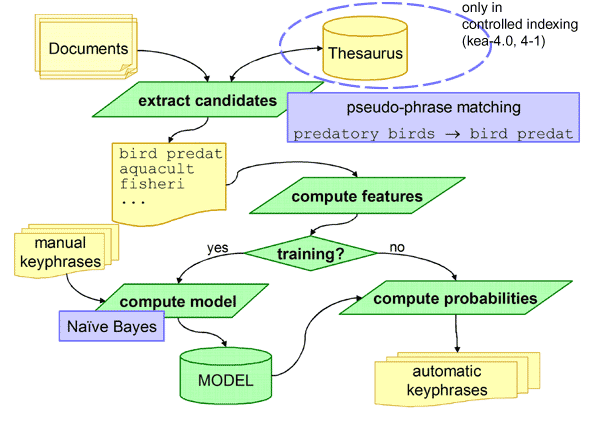
\includegraphics[scale=1]{res/kea_diagram.png}
\caption{Schema di Kea}
\label{fig:kea}
\end{figure}
